\documentclass[12pt, a4paper]{article}
\usepackage{fontspec}
\usepackage{xeCJK}
\usepackage{hyperref}
\setCJKmainfont{微軟正黑體}
\XeTeXlinebreaklocale "zh"
\XeTeXlinebreakskip = 0pt plus 1pt
\usepackage{enumerate}
\usepackage{graphicx}
\usepackage{amsmath}
\usepackage[tmargin = 4cm]{geometry}
\date{}
\title{\vspace{-3.0cm} Robotics : Assignment 3 \\ \vspace{0.5cm}}
\author{\textbf{Group 2} : \normalsize{r05922008 丁柏文\mbox{ }r05922084 韓翔宇} \\ \hspace{2.48cm} \normalsize{r05922146 葉興宇\mbox{ }b03902062 董文捷}}
\begin{document}
\maketitle
\begin{enumerate}

\item \textbf{The physical meaning of the intrinsic parameters} \\
The intrinsic parameters for \textit{Xiaomi 5} with \textit{Camera FV-5 Lite app} is \\ 
\begin{tabular}[t]{cc}
$f_x = 5.2527901518613203e+02$ & $f_y = 5.2423050665947335e+02$ \\ 
$c_x = 3.3348261217425255e+02$ & $c_y = 2.3490390416419061e+02$ \\
\end{tabular} \\
\vspace*{0cm} \\
In \href{http://docs.opencv.org/master/d4/d94/tutorial_camera_calibration.html}{Camera calibration With OpenCV}, the calibration is done with the help of the 
\href{http://docs.opencv.org/master/d9/d0c/group__calib3d.html#ga3207604e4b1a1758aa66acb6ed5aa65d}{\texttt{cv::calibrateCamera}} function, which finds the camera intrinsic and extrinsic parameters from several views of a calibration pattern.
The intrinsic parameters $f_x$, $f_y$, $c_x$, and $c_y$ is stored in the output 3x3 floating-point \texttt{cameraMatrix} with the form \texttt{cameraMatrix} = 
$\begin{bmatrix}
f_x & 0 & c_x \\
0 & f_y & c_y \\ 
0 & 0 & 1 \\
\end{bmatrix}$. \\
Those intrinsic parameters have their significant physical meanings in the camera model. We first consider a simple geometry camera model, \textit{pinhole camera model}, which describes the mathematical relationship between the coordinates of a 3D point and its projection onto the image plane. \\
\vspace*{0cm} \\
\includegraphics[scale = 0.6]{3_1.JPG} \\
\newpage
\includegraphics[scale = 0.66]{3_2.JPG} \\
By similarity of the triangles, we can get $\displaystyle \frac{x}{f} = \frac{X}{Z} \rightarrow x = f \frac{X}{Z}$ \\
Same relation holds for $y$, too. $\displaystyle \frac{y}{f} = \frac{Y}{Z} \rightarrow y = f \frac{Y}{Z}$ \\
Ideally, principal point $c$, the intersection point of the optical axis and the image plane, should be the center of the image. However, due to assembly error of the camera, the position of $c$ in image plane may located at $(c_x, c_y)$. Therefore, the relations become 
$\displaystyle x = f [\frac{X}{Z}] + c_x \mbox{ }\mbox{ } y = f [\frac{Y}{Z}] + c_y$ \\
Furthermore, since we need to use pixel as a unit in the image plane, and the aspect ratio of a pixel may not be 1, that is to say, a pixel is a rectangle rather than a square, we use $s_x$ and $s_y$ to rewrite the relation as \\
$\displaystyle x = f [\frac{X}{Z}] \cdot s_x + c_x \mbox{ }\mbox{ } y = f [\frac{Y}{Z}] \cdot s_y + c_y$ \\
Let $\displaystyle f \cdot s_x = f_x$ and $\displaystyle f \cdot s_y = f_y$, we finally get 
$\displaystyle x = f_x [\frac{X}{Z}] + c_x \mbox{ }\mbox{ } y = f_y [\frac{Y}{Z}] + c_y$

\item \textbf{The effect of} \href
{http://docs.opencv.org/master/da/d54/group__imgproc__transform.html#ga69f2545a8b62a6b0fc2ee060dc30559d}{\textbf{\texttt{cv::undistort}}} \\
In \textit{pinhole camera model}, the camera aperture is described as a point. Nevertheless, we use lenses to focus light and reduce the exposure time in reality. Lenses can distort images, especially at short focal length. \\
\newpage
\hspace*{-1cm}
\begin{tabular}[t]{ccc}
\includegraphics[scale = 0.25]{images2/1.jpg} & \includegraphics[scale = 0.3]{arrow.jpg} &\includegraphics[scale = 0.25]{1.jpg} \\
\includegraphics[scale = 0.25]{images2/2.jpg} & \includegraphics[scale = 0.3]{arrow.jpg} &\includegraphics[scale = 0.25]{2.jpg} \\
\includegraphics[scale = 0.25]{images2/3.jpg} & \includegraphics[scale = 0.3]{arrow.jpg} &\includegraphics[scale = 0.25]{3.jpg} \\
\includegraphics[scale = 0.25]{images2/4.jpg} & \includegraphics[scale = 0.3]{arrow.jpg} &\includegraphics[scale = 0.25]{4.jpg} \\
\includegraphics[scale = 0.25]{images2/5.jpg} & \includegraphics[scale = 0.3]{arrow.jpg} &\includegraphics[scale = 0.25]{5.jpg} \\
\end{tabular}
\newpage
\hspace*{-1cm}
\begin{tabular}[t]{ccc}
\includegraphics[scale = 0.25]{images2/6.jpg} & \includegraphics[scale = 0.3]{arrow.jpg} &\includegraphics[scale = 0.25]{6.jpg} \\
\includegraphics[scale = 0.25]{images2/7.jpg} & \includegraphics[scale = 0.3]{arrow.jpg} &\includegraphics[scale = 0.25]{7.jpg} \\
\includegraphics[scale = 0.25]{images2/8.jpg} & \includegraphics[scale = 0.3]{arrow.jpg} &\includegraphics[scale = 0.25]{8.jpg} \\
\includegraphics[scale = 0.25]{images2/9.jpg} & \includegraphics[scale = 0.3]{arrow.jpg} &\includegraphics[scale = 0.25]{9.jpg} \\
\includegraphics[scale = 0.25]{images2/10.jpg} & \includegraphics[scale = 0.3]{arrow.jpg} &\includegraphics[scale = 0.25]{10.jpg} \\
\end{tabular}
\newpage
\hspace*{-1cm}
\begin{tabular}[t]{ccc}
\includegraphics[scale = 0.25]{images2/11.jpg} & \includegraphics[scale = 0.3]{arrow.jpg} &\includegraphics[scale = 0.25]{11.jpg} \\
\includegraphics[scale = 0.25]{images2/12.jpg} & \includegraphics[scale = 0.3]{arrow.jpg} &\includegraphics[scale = 0.25]{12.jpg} \\
\includegraphics[scale = 0.25]{images2/13.jpg} & \includegraphics[scale = 0.3]{arrow.jpg} &\includegraphics[scale = 0.25]{13.jpg} \\
\includegraphics[scale = 0.25]{images2/14.jpg} & \includegraphics[scale = 0.3]{arrow.jpg} &\includegraphics[scale = 0.25]{14.jpg} \\
\includegraphics[scale = 0.25]{images2/15.jpg} & \includegraphics[scale = 0.3]{arrow.jpg} &\includegraphics[scale = 0.25]{15.jpg} \\
\end{tabular}
\newpage
\hspace*{-1cm}
\begin{tabular}[t]{ccc}
\includegraphics[scale = 0.25]{images2/16.jpg} & \includegraphics[scale = 0.3]{arrow.jpg} &\includegraphics[scale = 0.25]{16.jpg} \\
\includegraphics[scale = 0.25]{images2/17.jpg} & \includegraphics[scale = 0.3]{arrow.jpg} &\includegraphics[scale = 0.25]{17.jpg} \\
\includegraphics[scale = 0.25]{images2/18.jpg} & \includegraphics[scale = 0.3]{arrow.jpg} &\includegraphics[scale = 0.25]{18.jpg} \\
\includegraphics[scale = 0.25]{images2/19.jpg} & \includegraphics[scale = 0.3]{arrow.jpg} &\includegraphics[scale = 0.25]{19.jpg} \\
\includegraphics[scale = 0.25]{images2/20.jpg} & \includegraphics[scale = 0.3]{arrow.jpg} &\includegraphics[scale = 0.25]{20.jpg} \\
\end{tabular}
\newpage
\hspace*{-1cm}
\begin{tabular}[t]{ccc}
\includegraphics[scale = 0.25]{images2/test.jpg} & \includegraphics[scale = 0.3]{arrow.jpg} &\includegraphics[scale = 0.25]{21.jpg} \\
\end{tabular}
\\
For the distortion \texttt{OpenCV} takes into account the radial and tangential factors. Radial distortion occurs when light rays bend more near the edges of a lens than they do at its optical center, most visible when taking pictures of vertical structures having straight lines which then appear curved. For the radial factor \texttt{OpenCV} uses the following formula \\
$\displaystyle x_{distorted} = x(1+k_1r^2+k_2r^4+k_3r^6)\mbox{ }\mbox{ }y_{distorted}=y(1+k_1r^2+k_2r^4+k_3r^6)$ \\
On the other hand, tangential distortion occurs because the image taking lenses are not perfectly parallel to the image plane. It can be represented via the formulas \\
$\displaystyle x_{distorted}=x+[2p_1xy+p_2(r^2+2x^2)]\mbox{ }\mbox{ }y_{distorted}=y+[p_1(r^2+2y^2)+2p_2xy]$ \\
The distortion coefficients are also calculated in \texttt{cv::calibrateCamera}, presented as 
\texttt{distCoeffs} = $\displaystyle (k_1\mbox{ }k_2\mbox{ }p_1\mbox{ }p_2\mbox{ }k_3)$. 
With \texttt{cameraMatrix} and \texttt{distCoeffs}, \texttt{cv::undistort} is able to transform an image to compensate for lens distortion.
In our result, we have $k_1 = 7.5350825654120113e-01$, $k_2 = -6.8824480883938541e+00$, $p_1 = 0$, $p_2 = 0$, $k_3 = 1.6336663151773003e+01$. The undistorted images are obviously concave, trying to fix the radial distortion.
\item \textbf{The division of work within our team}
\begin{itemize}
\item r05922008 資工碩一\mbox{ }丁柏文 : \textbf{Part B} program.
\item r05922084 資工碩一\mbox{ }韓翔宇 : \textbf{Part A} program.
\item r05922146 資工碩一\mbox{ }葉興宇 : Report \textbf{Part A (5)}.
\item b03902062 資工三\mbox{ }董文捷 : Report \textbf{Part A (4)}.
\end{itemize}

\item \textbf{Environment} \\
\texttt{ubuntu 16.04}, \texttt{OpenCV 3.1} 
\item \textbf{References} 
\begin{enumerate}[(1)]
\item Figures from \href{https://www.comp.nus.edu.sg/~cs4243/lecture/camera.pdf}{Camera Models and Imaging} 
\item \href{http://wycwang.blogspot.tw/2012/09/camera-calibration-part-1-camera-model.html}{攝像頭校正 camera calibration - part 1 camera model}
\item \href{http://wycwang.blogspot.tw/2012/10/camera-calibration-part-2-calibration.html}{攝像頭校正 camera calibration - part 2 calibration}
\item \href{https://www.mathworks.com/help/vision/ug/camera-calibration.html?requestedDomain=www.mathworks.com}{What Is Camera Calibration?}
\end{enumerate}

\end{enumerate}
\end{document}